\chapter{MATERIALS AND METHODS}
In this thesis, we predict the binding affinity score of drug-target pairs by using heterogeneous graphs generated with the existing and extracted information of chemicals and proteins. To do so, we divide the study in to 5 stages; in Stage 1, we compiled data from databases listed in Chapter \ref{chapter:dataset_preparation}, in Stage 2, we assembled these data as described in Section \ref{section:data_assembling} and extract useful information from them, in Stage 3, we created homogeneous and heterogeneous graphs using assembled data, in Stage 4, we learned the distributional vector representations of proteins and ligands using homogeneous and heterogeneous graphs with and without several language models, and finally in Stage 5, we predict the affinity scores of drug-target pairs, and  evaluate the performance of our model.

\section{Dataset Compilation}
For the chemicals, we employ six databases and extract drug-related information such as unique IDs (InChI, CID, and DrugBank ID), SMILES strings, interacting drugs, interacting targets, side effects, and diseases. For the proteins, we used four databases and extract protein-related information such as unique IDs (Entrez Gene ID, and UniProt ID), amino acid sequences, interacting proteins, interacting drugs, and diseases. Figure \ref{fig:databases} shows these eight databases with the corresponding extracted information. 

\begin{figure}
    \centering
        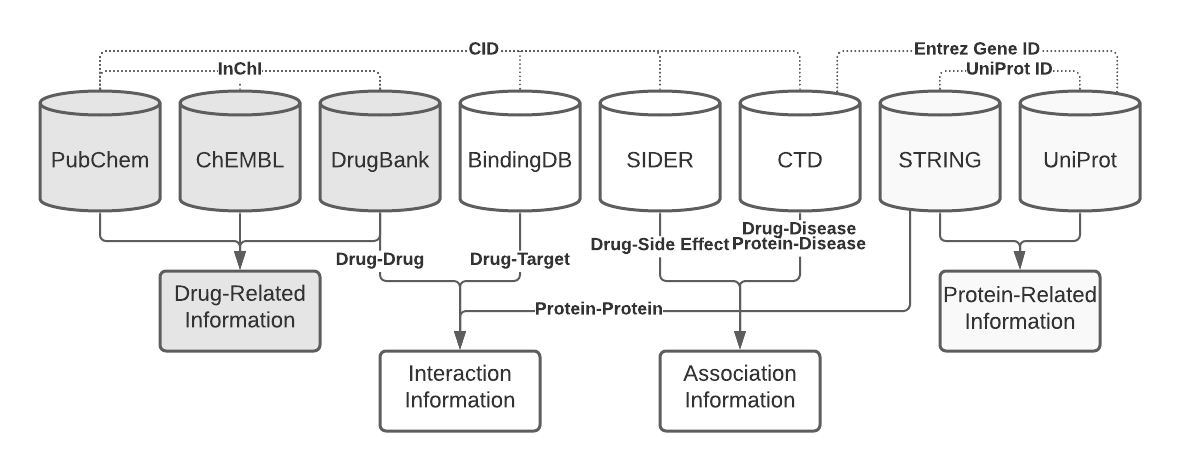
\includegraphics[width=\linewidth]{chapters/materials_and_methods/figures/databases.png}
    \caption{Compiled Databases.}
    \label{fig:databases}
\end{figure}


% TO DO: Which information is used, jaccard vs also, lm
\section{Data Assembling}
\label{section:data_assembling}
Our idea was to represent chemicals and proteins better. Therefore, we compiled chemical and proteins related data from several online databases. And the challenging task was to assemble these compiled large data. For that purpose we analyze the available information in above mentioned databases and and map related information using common data. Figure \ref{fig:databases} shows used databases and the mapping IDs between corresponding databases.

\subsection{Chemical Related Information}
DrugBank, PubChem, and ChEMBL databases are the main resources of chemicals and we mainly focus on them. As an initial step we compile 14.350 drugs from DrugBank and retrieve their DrugBank IDs and InChI (International Chemical Identifier) Keys. Using InChI keys, we map the data in DrugBank to PubChem and ChEMBL databases and able to get the information about 10.935 distinct drugs. With 10.935 drugs, we extract 2.196.820 drug-drug relation information from DrugBank database. Using the PubChem CID (Compound ID number) information available at PubChem database, we map the PubChem to SIDER and CTD databases. From SIDER database, we extract 5452 distinct side effects and 115.871 drug-side effect association information for 1003 drugs. From CTD database, we extract 7086 distinct diseases and 995.654 drug-disease association information for 3387 drugs. Finally, using the InChI keys, we map DrugBank to ChEMBL and compile SMILES (Simplified molecular-input line-entry system) representations of 10.935 drugs. 

Apart from the already existing information we create a new relation, which we named as drug-drug similarity (DDS). Using the compiled SMILES representations of drugs from the ChEMBL (Davies et al., 2015) database, DDS data is obtained by calculating the similarity of these representations to each other according to the Jaccard Similarity Criterion. In order to find the similar SMILES sequences we used the Byte Pair Encoding (BPE) algorithm \cite{sennrich2015neural}. The BPE approach was utilized to identify the language unit vocabulary of chemicals. This method is commonly employed for discovering the tokens of a language, in the field of NLP. The BPE algorithm divided SMILES sequences into language units. Then, the similarity of the drugs was calculated in pairs according to the Jaccard Criterion using the formula given in Equation \ref{eq:jaccard}. By calculating the Jaccard Similarities of all drug-drug pairs, we obtained the values shown in Figure \ref{fig:dds}. Accordingly, drug pairs in the data set with a similarity value greater than $58$ were determined to be similar to each other with a threshold value was determined to cover at least $10\%$ of the whole data. In the end, we created 2.924.270 drug-drug similarity value for 6.963 distinct drugs.

\begin{equation}
    Jaccard (A, B) = \frac{A \cap  B}{ A \cup B} \times  100
\label{eq:jaccard}
\end{equation}

\begin{figure}
    \centering
        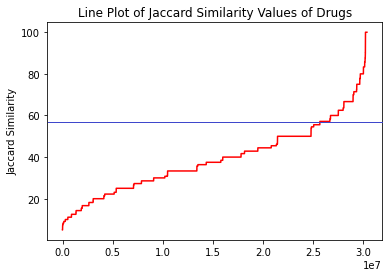
\includegraphics[width=0.5\linewidth]{chapters/materials_and_methods/figures/dds_line.png}
    \caption{Pairwise Drug-Drug Jaccard Similarities.}
    \label{fig:dds}
\end{figure}

%Given a corpus, all uni-characters are first considered as language units by the algorithm. The program then determines the total length of all pairs in the given text. The algorithm, now includes the most common two-character subsequences in the vocabulary. By treating each uni-characters in the vocabulary as a single character, this procedure continues until the goal vocabulary size is generated. The most frequently occurring subsequences of the necessary size are obtained when the method completes.

\subsection{Protein Related Information}
UniProt and STRING databases are main resources used in this thesis. We compile 505.250 proteins from the UniProt database and more specifically we compile 202.160 proteins belonging to the Homo sapiens, as well as their amino acid sequences. Using the UniProt ID from UniProt database, we map 18.876 proteins to STRING database, and extract 183.746 protein-protein interaction information. Finally, using the UniProt ID and Entrez Gene ID we map UniProt database to CTD and extract 32.495 protein-disease association information for 32.169 proteins and 126 distinct diseases.

Similar to the chemicals, besides the already existing protein-related information we create a new relation, which we named as protein-protein similarity (PPS). Using the compiled amino acid  sequences of proteins from the UniProt database, PPS data is obtained by calculating the similarity of these representations to each other according to the Jaccard Similarity Criterion. Again, we employ BPE algorithm to find the language units of protein sequences. Then, the similarity of the proteins was calculated in pairs according to the Jaccard Criterion using the formula given in Equation \ref{eq:jaccard}. By calculating the Jaccard Similarities of all protein-protein pairs, we obtained the values shown in Figure \ref{fig:pps}. Accordingly, protein pairs in the data set with a similarity value greater than $9$ were determined to be similar to each other with a threshold value was determined to cover at least $11\%$ of the whole data. In the end, we created 528 protein-protein similarity value for 465 distinct proteins.


\begin{figure}
    \centering
        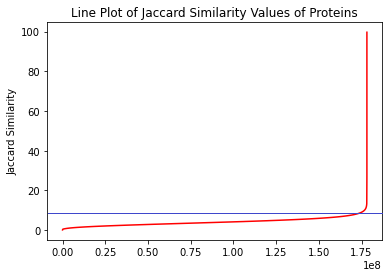
\includegraphics[width=0.5\linewidth]{chapters/materials_and_methods/figures/pps_line.png}
    \caption{Pairwise Protein-Protein Jaccard Similarities.}
    \label{fig:pps}
\end{figure}

\section{Graph Creation}
% TO DO: Insert node edge numbers, types
% pos and neg edge sampling
\subsection{Homogeneous Graphs}



\subsection{Heterogeneous Graphs}


\section{Learning Distributional Vector Representations}
Machine learning on graph structured data is a ubiquitous task and one of the challenges of this task is to find a way to represent the structure itself and the information it holds so that it can be easily interpreted by mostly used machine learning models. In this thesis, we employ metaPath2Vec \cite{dong2017metapath2vec} model and learn the graph-based distributional representation vectors that reflect the semantic connections in the graph for nodes and edges and finally represent data that cannot be expressed in Euclidean space as a graph.

MetaPath2Vec uses \textit{priori} paths as its basic operating principle. It evaluates different types of edge relations while finding meta paths, that is, paths going from one node to another node, provided that they do not repeat it again, and makes semantic inferences using these edges and uses them in vector representations.



% cosine similarity ile val evaluation
% hepsinin sonuclari



\section{WiderDeepDTA}
In WideDeepDTA, we empowered heterogeneous networks using language models. 
% explain used machines.


\begin{figure}
    \centering
        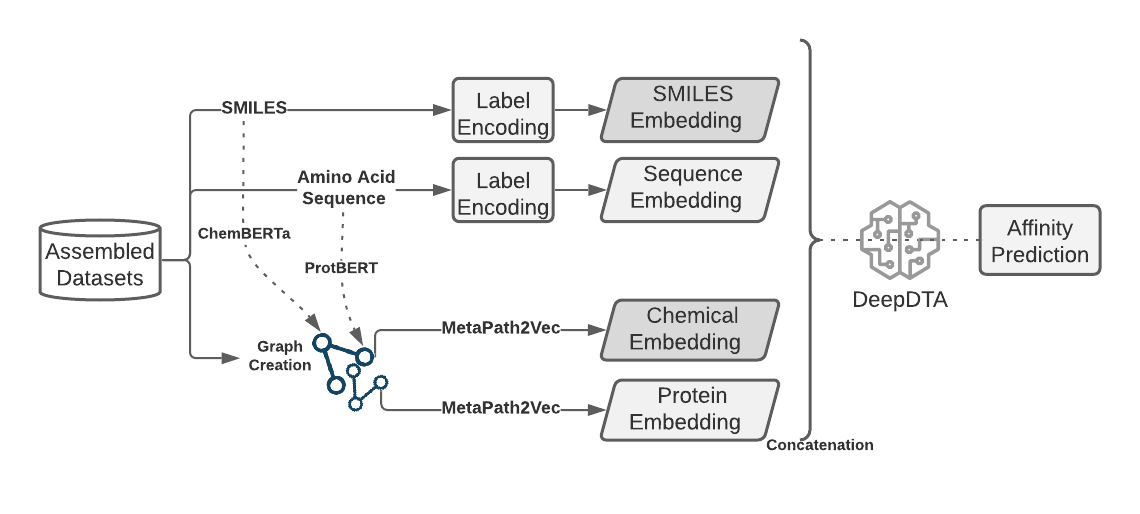
\includegraphics[width=\linewidth]{chapters/materials_and_methods/figures/WiderDeepDTA.png}
    \caption{WideDeepDTA Summarized.}
    \label{fig:widerdeepdta}
\end{figure}


\begin{figure}
    \centering
        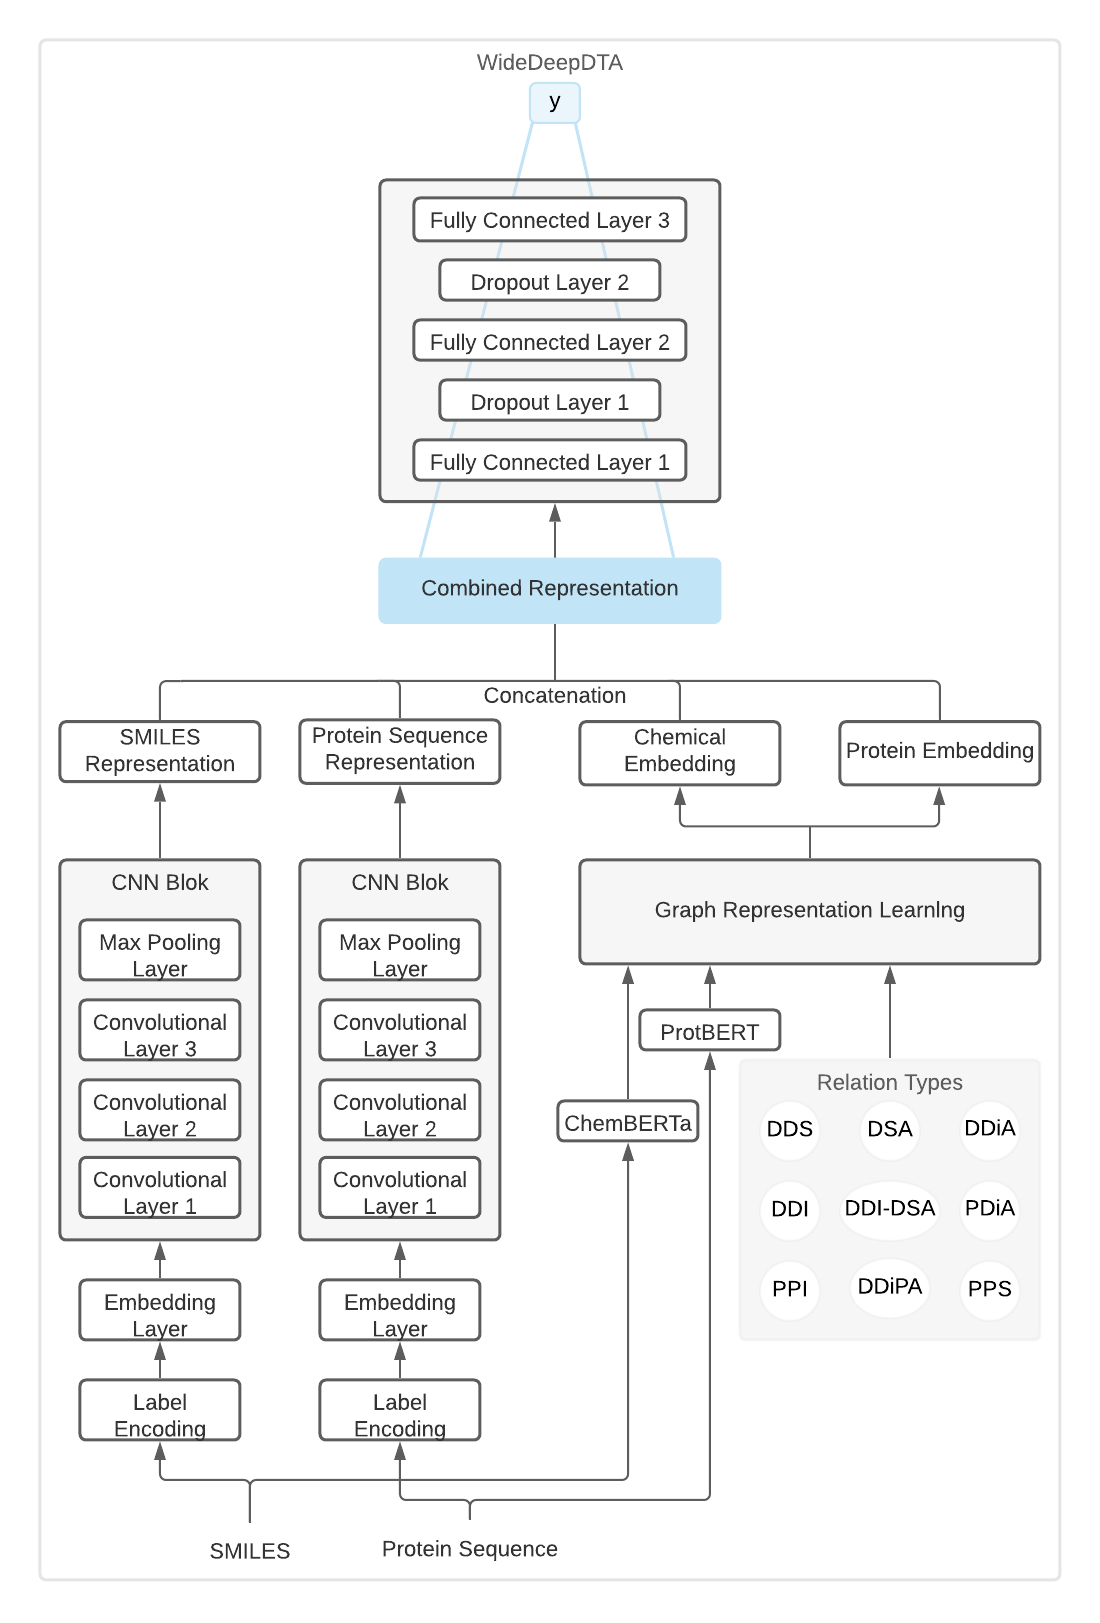
\includegraphics[width=\linewidth]{chapters/materials_and_methods/figures/WiderDeepDTA Model.png}
    \caption{WideDeepDTA in Details.}
    \label{fig:widedeepdtamodel}
\end{figure}